\chapter{Applicazione della teoria dei fili}\label{chapter:applicazione_teoria_fili}
\begin{figure}

  \centering
  
  \begin{tikzpicture}[spy using outlines={circle,red,dashed, magnification=4,size=9cm, connect spies}]
   
     \draw [-latex] (0,0) -- (9.5,0) node [below] {$x$};
     \draw [-latex] (0,0) -- (0,4) node [left] {$y$};
     \node at (0,0) [below left] {$O$};
 
     \draw [thick] (1,2) parabola  bend (4.5,1) (8,2);
     \node at (1,2) [above left] {$A$};
     \node at (8,2) [above right] {$B$};
 
     \draw [very thick, red] (1,0) -- (8,0);
     \node [color = red] at (4.5,0) [below] {$\lambda>0$};
 
     \foreach \x in {1,1.2,...,8} 
     \draw (\x,0) -- (\x, 4/49*\x*\x - 36/49*\x + 130/49);
   
   \point {a}{1}{2.5};
   \point {b}{8}{2.5};
   \lineload {1}{a}{b}[.5][.5][.09];
   \dimensioning {1}{a}{b}{-1}[$L$];
 
   \node at (4.5, 3.6) {$\overline{f}(s)$};
   \draw [-latex, thick] (9,3)--(9,2) node [right] {$\overline{g}$};


   \begin{scope}[shift={(-0.2,-5.8)}]
    \node at (.4,2.5) {$P(s)$};
    \node at (6.5,1.2) {$P(s+ds)$};
    \draw [-latex, very thick, red] (3.2,-3.4) --+(0,-1) node [above right] {$-\lambda\,g\,dx\,\hat{e}_2$};
    \draw [very thick, -latex] (3.2, 3.3) node [below right] {$\overline{f}\,ds$}--+ (0,-1.8);

    \end{scope}

   
   \spy on (3, .8) in node  at (3,-6);

   


  \end{tikzpicture}
  
  \caption{Problema del ponte sospeso}
  \label{fig:problema_ponte_sospeso}
  
  
  
 \end{figure}

La teoria dei fili, trattata nel capitolo precedente, può essere applicata a problemi reali. 
In particolare, in questo capitolo, si tratteranno i seguenti casi:
\begin{itemize}
 \item equazione dei ponti sospesi;
 \item catenaria omogenea;
 \item filo soggetto a sollecitazioni distribuite nulle;
 \item filo soggetto a carichi concentrati.
\end{itemize}

\section{Equazione dei ponti sospesi}
\label{section:equazione_ponti_sospesi}
Il caso in esame è descritto da un'asta rigida rettilinea e omogenea di lunghezza $L$ e densità lineare $\lambda>0$, collegata a una fune inestensibile ($E\,A \to\infty$) e perfettamente flessibile ($E\,I=0$) mediante una serie di tiranti verticali. La fune è fissata agli estremi $A$ e $B$ con appositi vincoli (figura~\ref{fig:problema_ponte_sospeso}). 

Si consideri un sistema di riferimento cartesiano nel piano $Oxy$ in modo tale che l'asta rigida giaccia sull'asse delle ascisse; inoltre, si consideri la gravità come $\overline{g} = - g\,\hat{e}_2$.

Si ricerca la configurazione di equilibrio e il valore delle reazioni vincolari agli estremi che garantiscano l'equilibrio.

Lo scopo dei tiranti è quello di trasmettere le forze agenti sull'asta (in questo caso il peso proprio) alla fune. Postulando un numero di tiranti elevato si può immaginare che la fune sia soggetta a una distribuzione di forze continua di densità $\overline{f}(s)$.

Sia $s$ l'ascissa curvilinea con origine nell'estremo $A$; in funzione dell'ascissa è possibile scrivere la parametrizzazione della curva funicolare nel sistema di riferimento scelto
\[
 P(s) - O = x(s)\,\hat{e}_1 + y(s)\,\hat{e}_2
\]
valida per ogni $s\in[s_1, s_2]$.

Si consideri un tratto infinitesimo di filo di lunghezza $ds$; questo è sottoposto alla forza peso del tratto di asta sottostante. In particolare
\[
 \overline{f}\,ds = -\lambda\,g\left(x(s+ds) - x(s)\right)\,\hat{e}_2 
\]
ed espandendo in serie di Taylor il termine $x(s+ds)$ nell'intorno di $x(s)$ si ricava
\[
 x(s+ds)\simeq x(s) + \dfrac{dx}{ds}(s)\,ds + o(ds^2)
\]

Sostituendo, trascurando i termini di ordine superiore, si ottiene
\[
 \overline{f}\,ds = -\lambda\,g\left(x(s) + \dfrac{dx}{ds}(s)\,ds - x(s)\right)\,\hat{e}_2 = -\lambda\,g\,\dfrac{dx}{ds}(s)\,ds\,\hat{e}_2 
\]
che è il vettore risultante agente sul tratto di filo $ds$. Per ricavare la densità di forza agente sulla fune infinitesima è sufficiente dividere per $ds$
\[
 \overline{f}(s) = -\lambda\,g\,\dfrac{dx}{ds}(s)\,\hat{e}_2
\]

Essendo $\overline{f}$ diretto lungo la sola direzione $\hat{e}_2$ il problema ricade nel caso studiato al capitolo~2 nel paragrafo~\ref{section:forze_continue_parallele} a pagina~\pageref{section:forze_continue_parallele}. 
Risultano, allora, applicabili le due equazioni \eqref{eq:sistema_terna_standard} propriamente riscritte nel caso specifico per la costante $c$ strettamente positiva. 

Ricordando che 
\[
 \dfrac{dx}{ds} = \left(\dfrac{ds}{dx}\right)^{-1} = \left[1+\left(\dfrac{dy}{dx}\right)^2\right]^{-1/2}
\]
e sostituendo nella relazione della forza $f$
\[
 f = -\lambda\,g\,\dfrac{dx}{ds} = -\lambda\,g\left[1+\left(\dfrac{dy}{dx}\right)^2\right]^{-1/2}
\]

L'equazione differenziale finale \eqref{eq:cartesiana_funicolare}, sostituendo a $f$ la relazione appena calcolata, diventa
\begin{equation*}
 c\,\left[1+ \left(\dfrac{dy}{dx}\right)^2\right]^{-1/2}\,\dfrac{d^2 y}{dx^2} -\lambda\,g\left[1+\left(\dfrac{dy}{dx}\right)^2\right]^{-1/2} = 0
\end{equation*}
ed essendo $\left[1+\left(\frac{dy}{dx}\right)^2\right]^{-1/2}>0\quad\forall x\in\mathbb{R}$ si ricava una equazione differenziale del secondo ordine nella coordinata $x$
\begin{equation}
 \label{eq:equazione_differenziale_ponte_sospeso}
 c\,\dfrac{d^2y}{dx^2} - \lambda\,g = 0\qquad \Longrightarrow\qquad \dfrac{d^2y}{dx^2} = \dfrac{\lambda\,g}{c}
\end{equation}
detta \emph{equazione dei ponti sospesi} di soluzione generale 
\begin{equation}
\label{eq:equazione_ponte_sospeso}
 y(x) = \dfrac{\lambda\,g}{2 c}\,x^2 + a\,x+ b
\end{equation}
ove $a,b,c >0$ sono costanti arbitrarie. La soluzione è una curva parabolica con asse verticale e concavità verso l'alto.

Le costanti $a,b$ e $c$ si determinano imponendo la posizione degli estremi $A$ e $B$
\[
 y(x_1) = y_1 \qquad y(x_2)=y_2
\]
e la lunghezza totale della fune
\[
 L = \int_{x_1}^{x_2} \sqrt{1+y'(x)^2}\,dx
\]
nonché assegnando la ascissa curvilinea in un estremo
\[
 s(x_1) = s_1
\]

Noti i parametri è possibile calcolare la tensione nel filo usando la \eqref{eq:calcolo_tensione}
\[
 T(x) = c\left[1+\left(\dfrac{dy}{dx}\right)^2\right]^{1/2} = c\left[1+\left(\dfrac{\lambda\,g}{c}\,x + a\right)^2\right]^{1/2}
\]

In particolare, calcolando $T(x_1)$ e $T(x_2)$ si ricavano le tensioni agli estremi che garantiscano l'equilibrio e quindi le reazioni vincolari in $A$ e $B$
\begin{align*}
 &T_A = -T(x_1) = -c\left[1+\left(\dfrac{\lambda\,g}{c}\,x_1 + a\right)^2\right]^{1/2}\\
 &T_B = -T(x_2) = -c\left[1+\left(\dfrac{\lambda\,g}{c}\,x_2 + a\right)^2\right]^{1/2}
 \end{align*}
 
 \section{Catenaria omogenea}
 \begin{figure}
  \centering
  
  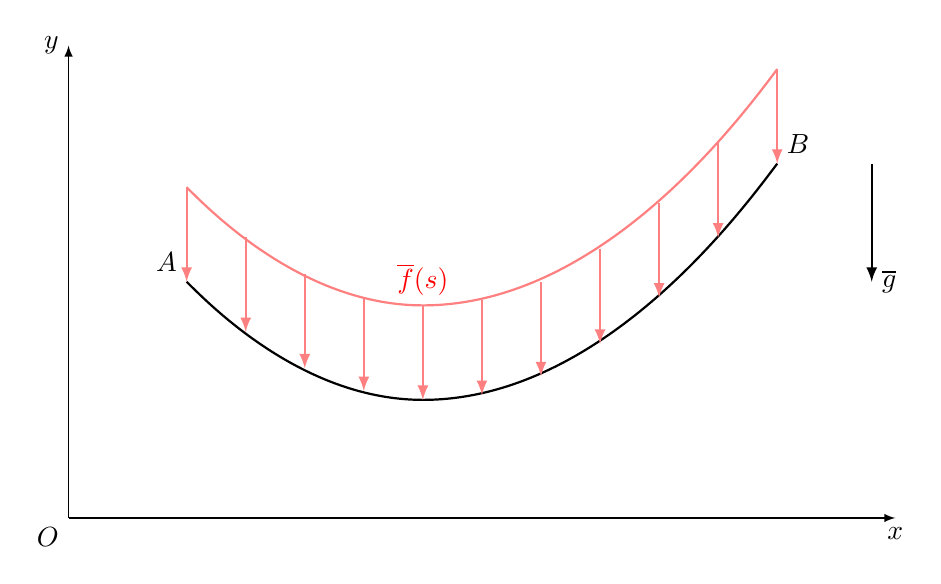
\begin{tikzpicture}[scale = 1.5]
   
     \draw [-latex] (0,0) -- (7,0) node [below] {$x$};
     \draw [-latex] (0,0) -- (0,4) node [left] {$y$};
     \node at (0,0) [below left] {$O$};
 
     \draw [thick] (1,2) parabola  bend (3,1) (6,3);
     \node at (1,2) [above left] {$A$};
     \node at (6,3) [above right] {$B$};

     \foreach \x in {1,1.5,...,6}
     \draw [red!50, latex-, thick] (\x, \x*\x*7/30 - \x*43/30 +16/5) --+ (0,.8);

     \begin{scope}[shift = {(0,.8)}]
      \draw [red!50, thick] (1,2) parabola  bend (3,1) (6,3);
      \node at (3,1) [color = red, above] {$\overline{f}(s)$};
     \end{scope}
 
   \draw [-latex, thick] (6.8,3)--(6.8,2) node [right] {$\overline{g}$};

  \end{tikzpicture}
  
  \caption{Problema della catenari omogenea}
  \label{fig:problema_catenaria_omogenea}
  
  
  
 \end{figure}

 Il problema della catenaria omogenea vuole studiare la configurazione di equilibrio di una fune di densità lineare $\lambda$ vincolata agli estremi $A$ e $B$ e soggetta esclusivamente al proprio peso (figura~\ref{fig:problema_catenaria_omogenea}). 
 
 Il sistema di riferimento da scegliere è quello cartesiano destro $Oxyz$ dove la verticale coincide con l'asse $Oy$. Per semplicità si suppone che la fune giaccia nel piano $Oxy$.
 
 Come nel caso del ponte sospeso, si può parametrizzare la curva in funzione dell'ascissa curvilinea $s$ nel seguente modo
 \[
  P(s) - O = x(s)\,\hat{e}_1 + y(s)\,\hat{e}_2,\qquad s\in[s_1, s_2]
 \]
 
Il tratto di filo infinitesimo che va dal generico punto $P(s)$ a $P(s+ds)$ sarà soggetto al proprio peso, quindi
\[
 \overline{f}\,ds = -\lambda\,g\,ds\,\hat{e}_2
\]
dove $\overline{f}$ è la densità di forza per unità di lunghezza, che vale
\[
 \overline{f} = -\lambda\,g\,\hat{e}_2
\]

Anche in questo caso sono applicabili le formule per forze di medesima direzione sostituendo $f$ con $-\lambda\,g$.

Considerando la costante $c>0$, l'equazione di equilibrio \eqref{eq:cartesiana_funicolare} è
\[
 \left[1+\left(\dfrac{dy}{dx}\right)^2\right]^{-1/2}\,\dfrac{d^2y}{dx^2} - \dfrac{\lambda\,g}{c} = 0
\]

Posto $y' = \frac{dy}{dx}(x)$ si può risolvere l'equazione differenziale con il metodo di separazione delle variabili.
\[
 \left(1+y'^2\right)^{-1/2}\,\dfrac{dy'}{dx} - \dfrac{\lambda\,g}{c} = 0 \quad \Longrightarrow\quad \dfrac{dy'}{\left(1+y'^2\right)^{1/2}} = \dfrac{\lambda\,g}{c}\,dx
\]

Integrando in maniera indefinita si ottiene
\begin{align*}
 \int \dfrac{dy'}{\left(1+y'^2\right)^{1/2}} =&\int \dfrac{\lambda\,g}{c}\,dx\\
 =& \dfrac{\lambda\,g}{c}\,x + a
\end{align*}
dove $a$ è una costante arbitraria.

Il termine a primo membro si risolve con il metodo di sostituzione, ponendo $y' = \sinh \eta$; il differenziale diventa
\[
 \dfrac{dy'}{d\eta} = \cosh\eta \quad \Longrightarrow\quad dy' = \cosh\eta\,d\eta
\]

Sostituendo nell'integrale, essendo inoltre $\cosh^2\eta - \sinh^2\eta = 1$
\[
 \int \dfrac{dy'}{\left(1+y'^2\right)^{1/2}} = \int \dfrac{\cosh\eta}{(1+\sinh^2\eta)^{1/2}}\,d\eta = \int \dfrac{\cosh\eta}{\cosh\eta}\,d\eta = \int d\eta = \eta
\]

Allora risulta
\[
\eta = \dfrac{\lambda\,g}{c}\,x + a    
\]
e sostituendo nella relazione imposta precedentemente
\[
\dfrac{dy}{dx}(x) = y'(x) = \sinh \eta = \sinh\,\left(\dfrac{\lambda\,g}{c}\,x + a\right) 
\]

Integrando in modo indefinito nella variabile $x$ si calcola la funzione $y(x)$ che conduce alla parametrizzazione della funicolare, detta \emph{catenaria omogenea}
\begin{equation}
\label{eq:equazione_catenaria_omogenea}
y(x) = \dfrac{c}{\lambda\,g}\,\cosh\left(\dfrac{\lambda\,g}{c}\,x +a\right) + b
\end{equation}
dove $a,b,c>0$ sono le tre costanti che devono essere calcolate imponendo le coordinate degli estremi $y(x_1) = y_1$, $y(x_2) = y_2$ e la lunghezza della fune
\[
  L = \int_{x_1}^{x_2} \sqrt{1+y'(x)^2}\,dx  
\]

Sostituendo il valore di $y'(x)$ calcolato poco sopra
\begin{align*}
 L =& \int_{x_1}^{x_2} \left[1+\sinh^2\left(\dfrac{\lambda\,g}{c}\,x +a\right)\right]^{1/2}\,dx\\
  =& \int_{x_1}^{x_2} \cosh\left(\dfrac{\lambda\,g}{c}\,x +a\right)\,dx = \dfrac{c}{\lambda\,g}\left[\sinh\left( \dfrac{\lambda\,g}{c}\,x +a\right)\right]_{x_1}^{x_2}
\end{align*}

Una volta calcolati i valori delle costanti $a, b$ e $c$ è possibile studiare la curva \eqref{eq:equazione_catenaria_omogenea}. Le derivate prima e seconda, rispettivamente, valgono
\[
\begin{cases}
 y'(x) = \sinh\left(\dfrac{\lambda\,g}{c}\,x +a\right)\\
 y''(x) = \dfrac{\lambda\,g}{c}\,\cosh\left(\dfrac{\lambda\,g}{c}\,x + a\right) \geq \dfrac{\lambda\,g}{c}\geq 0\quad \forall x \in[x_1, x_2] 
 \end{cases}
\]

\begin{figure}
  \centering
  
  \begin{tikzpicture}
    \begin{axis}[
      legend style = {at= {(0.5,-.1)}, anchor = north},
      axis x line = center,
      axis y line = left,
      xlabel=$x$,
      ylabel=$y(x)$,
      xtick=\empty,
      ytick=\empty,
      domain=-2:2
      ]

\addplot[draw] {cosh(\x)};
\addlegendentry{$ y(x)= \cosh x$};
    \end{axis}

  \end{tikzpicture}
   \caption{Andamento della funzione coseno iperbolico}
   \label{fig:andamento_coseno_iperbolico}
  
 \end{figure}

Dalla derivata seconda si può constatare che la funicolare ha concavità rivolta verso l'alto, mentre, dalla derivata prima si possono studiare i punti critici
\[
 0 = \sinh\left(\dfrac{\lambda\,g}{c}\,x +a\right) \quad \Longleftrightarrow \quad x = -\dfrac{c\,a}{\lambda\,g}
\]
essendo $\sinh(0) = 0$.

Plottando il grafico della funzione coseno iperbolico (figura~\ref{fig:andamento_coseno_iperbolico}), si può notare una certa somiglianza con la funicolare derivante dall'equazione dei ponti sospesi.

Traslando orizzontalmente la catenaria di un valore $\xi\in\mathbb{R}$ dal punto critico 
\[x = -\dfrac{c\,a}{\lambda\,g} + \xi\]
l'equazione cartesiana, ora scritta in funzione di $\xi$, assume la seguente forma
\[
 y(\xi) = b + \dfrac{c}{\lambda\,g}\cosh\left(\dfrac{\lambda\,g}{c}\,\xi\right)
\]

Espandendo in serie di Taylor fino al quarto ordine, nell'intorno di $\xi = 0$, il coseno iperbolico
\[
 y(\xi) = b + \dfrac{c}{\lambda\,g}\left[1 + \dfrac{1}{2}\left(\dfrac{\lambda\,g}{c}\,\xi\right)^2 + \dfrac{1}{24}\left(\dfrac{\lambda\,g}{c}\,\xi\right)^4 \right] + o\left(\dfrac{\lambda\,g}{c}\,\xi\right)^6
\]

Troncandola al secondo ordine, nell'intorno del punto critico, la funzione è ben approssimata da un arco di parabola (figura~\ref{fig:confronto_catenaria_parabola}).



\begin{figure}
  \centering
  
  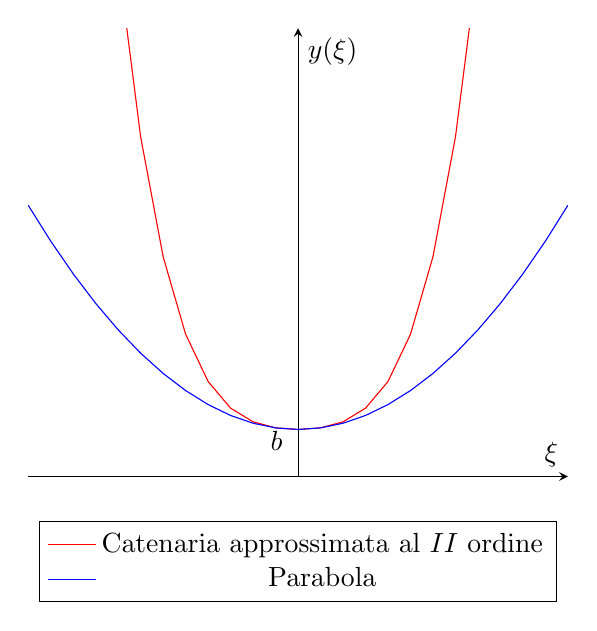
\begin{tikzpicture}
    \begin{axis}[
      legend style = {at= {(0.5,-.1)}, anchor = north},
      axis x line = center,
      axis y line = center,
      xlabel=$\xi$,
      ylabel=$y(\xi)$,
      xtick=\empty,
      ytick=\empty,
      ymin=0, 
      xmin = -5, 
      xmax = 5,
      ymin= 0,
      ymax=100,
      ytick = {10.5},
      yticklabel = $b$,
      yticklabel style = {yshift = -.15cm}
      ]

\addplot[draw, red] {10.5+2*\x*\x + (1/24)*16*(\x)^4};
\addlegendentry{Catenaria approssimata al $II$ ordine};

\addplot[draw, blue] {10.5 + 2*\x*\x };
\addlegendentry{Parabola};
    \end{axis}

  \end{tikzpicture}
  \caption{Confronto tra catenaria approssimata e parabola}
  \label{fig:confronto_catenaria_parabola}
   
  
 \end{figure}
 
I primi studi eseguiti da Leonardo da Vinci e Galileo Galilei sulla teoria dei fili  facevano riferimento alla sola parabola. In particolare, la teoria di Galileo tratta da \emph{Discorsi e dimostrazioni matematiche} non era totalmente errata, data la buona approssimazione tra le due curve.

Il dibattito sulla catenaria portato avanti da Huygens condusse a una rivalutazione della parabola di Galileo, in quanto non perfettamente in grado di descrivere  la fune di un ponte sospeso, a vantaggio della catenaria.

Nell'applicazione ai ponti sospesi, però, l'approssimazione tra catenaria e parabola è sufficientemente accettabile, tenendo conto del fatto che la fune principale di un ponte sospeso è soggetta solo al proprio peso che risulta distribuito lungo il cavo in maniera uniforme, come visto nel paragrafo~\ref{section:equazione_ponti_sospesi}

%*************************************************************************
%************************************************************************ 
\section{Filo soggetto a sollecitazioni distribuite nulle}
Nel caso particolare in cui sul filo non agiscono forze distribuite ($\overline{f}=0$), l'equazione indefinita di equilibrio \eqref{eq:equzione_indefinita_equilibrio} diventa semplicemente
\[
 \dfrac{d}{ds}(T\,\vtau)= 0 \quad \Longrightarrow\quad T\,\vtau = cost.
\]
che è soddisfatta se e solo se $T=cost.$ e $\vtau = cost.$

La costanza del versore tangente, definito come
\[
 \vtau = \dfrac{dP}{ds}(s) = cost.
\]
consegue dal fatto che la parametrizzazione della funicolare descrive una retta
\[
 P(s) = P(s_0) + (s - s_0 )\,\vtau\qquad \forall s\in[s_1, s_2]
\]
con $s_0\in[s_1, s_2]$.

Le tensioni agli estremi $A$ e $B$, allora, hanno ugual modulo e direzione ma verso opposto, come raffigurato in figura~\ref{fig:tensioni_forza_nulla}

\begin{figure}
 \centering
 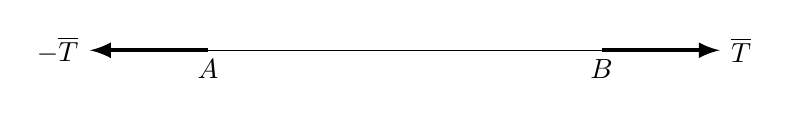
\begin{tikzpicture}
 \draw (0,0) node [below] {$A$} -- (5,0) node [below] {$B$};
 \draw [ultra thick, -latex] (0,0) --+ (-1.5,0) node [left] {$-\overline{T}$};
 \draw [ultra thick, -latex] (5,0) --+ (1.5, 0) node [right] {$\overline{T}$};
 \end{tikzpicture}
 \caption{Tensioni agli estremi nel caso di sollecitazioni distribuite nulle}
 \label{fig:tensioni_forza_nulla}
\end{figure}


\section{Filo soggetto a carichi concentrati}
Si consideri ora una fune di peso trascurabile soggetta a un sistema di forze concentrate $\overline{F}_0, \overline{F}_1, \dots,  \overline{F}_{N+1}$, applicate rispettivamente nei punti $P_0, P_1, \dots, P_{N+1}$ (dove $P_0$ e $P_{N+1}$ sono gli estremi della fune), di risultante nulla. 
\[
\left|\overline{R}\right| = \sqrt{\left(\sum_{i=0}^{N+1}F_{x_i}\right)^2 +\left(\sum_{i=0}^{N+1}F_{y_i}\right)^2} = 0
\]

Il sistema di riferimento adottato è quello cartesiano ortogonale con ipotesi che la fune si mantenga nel piano coordinato $Oxy$. Ne consegue che le forze puntuali hanno componente nulla lungo la direzione $z$.

Sono valide le equazioni indefinite di equilibrio \eqref{eq:sistema_terna_standard}, riscritte in maniera appropriata
\[
\begin{cases} 
  \dfrac{d}{ds}\left(T\,\dfrac{dx}{ds}\right) + R_x = 0\\[1.5ex]
  \dfrac{d}{ds}\left(T\,\dfrac{dy}{ds}\right) + R_y = 0
\end{cases}
\]
ed essendo $R_x = R_y = 0$
\begin{equation}
\label{eq:equazione_indefinita_equilibrio_concentrati}
\begin{cases} 
  \dfrac{d}{ds}\left(T\,\dfrac{dx}{ds}\right) = 0\\[1.5ex]
  \dfrac{d}{ds}\left(T\,\dfrac{dy}{ds}\right) = 0
\end{cases}
\end{equation}

Integrando in $s$ entrambe le equazioni
\[
\begin{cases} 
T\,\dfrac{dx}{ds} = c_1\\[1.5ex]
  T\,\dfrac{dy}{ds} = c_2
\end{cases}
\]
dove $c_1$ e $c_2$ sono costanti arbitrarie. Si può applicare quanto visto in precedenza nella teoria dei fili, essendo
\[
\begin{cases}
\overline{T}\cdot\hat{e}_1 = T\,\vtau\,\hat{e}_1 = T\,\dfrac{dP}{ds}\,\hat{e}_1 = T\,\dfrac{dx}{ds} = c_1\\[1.5ex]
\overline{T}\cdot\hat{e}_2 = T\,\vtau\,\hat{e}_2 = T\,\dfrac{dP}{ds}\,\hat{e}_2 = T\,\dfrac{dy}{ds} = c_2
\end{cases}
\]

Postulando le costanti $c_1$ e $c_2$ strettamente positive e considerando l'ascissa curvilinea $s(x)$ una funzione della coordinata $x$, si può scrivere
\[
\dfrac{ds}{dx} = \left.\left(\dfrac{dx}{ds}\right)^{-1}\right|_{s = s(x)} 
\]

Applicando quanto appena ricavato alla prima equazione integrata e isolando la derivata prima
\[
\dfrac{ds}{dx} = \left.\dfrac{T(s)}{c_1}\right|_{s = s(x)}
\]

Ora, ipotizzando $y = y(s(x))$
\[
\dfrac{dy}{dx} = \dfrac{dy}{ds}\,\dfrac{ds}{dx} = \dfrac{dy}{ds}\,\left(\dfrac{dx}{ds}\right)^{-1}
\]

La tensione può essere ricavata da
\[
T = c_1\left(\dfrac{dx}{ds}\right)^{-1}
\]
e sostituendolo nella equazione lungo $y$
\[
T\,\dfrac{dy}{ds} = c_1\left(\dfrac{dx}{ds}\right)^{-1}\,\dfrac{dy}{ds} = c_2
\]
e quindi, per quanto visto poco sopra
\begin{equation}
\label{eq:tratto_filo_costante}
\dfrac{dy}{dx} = c_3 = cost.\qquad \forall x\in[x_i, x_{i+1}]
\end{equation}
dove $c_3$ è una costante diversa da $c_1$ e $c_2$.

\begin{figure}
  \centering
  
  \begin{tikzpicture}
  \begin{scope}[shift = {(0,1)}]
  \draw[-latex] (0,0) node[below] {$O$} -- (7,0) node [below] {$x$};
  \draw[-latex] (0,0) -- (0,5) node [left] {$y$};
  \end{scope}
  
  \draw  (1,4) -- (2,3) -- (3,2.5) -- (4,2.5) -- (5,3) -- (6,4);
  
  \draw [-latex, very thick] (1,4) --+(-.5,1) node [right] {$\overline{F}_0$};
  \draw [latex-, very thick] (2,3) --+(.5,1) node [right] {$\overline{F}_1$}; 
  \draw [latex-, very thick] (3,2.5) --+(0,1) node [right] {$\overline{F}_2$}; 
  \draw [latex-, very thick] (4,2.5) --+(0,1) node [right] {$\overline{F}_3$};
  \draw [latex-, very thick] (5,3) --+(-0.5,1) node [right] {$\overline{F}_4$}; 
  \draw [-latex, very thick] (6,4) --+(0.5,1) node [right] {$\overline{F}_5$}; 
   



  \end{tikzpicture}

\caption{Configurazione della fune soggetta a 5 forze concentrate}
\label{fig:fune_forze_concentrate}
   
\end{figure}

La \eqref{eq:tratto_filo_costante} implica che, tra una sollecitazione puntuale e l'altra, il filo ha pendenza costante e risulta un segmento lineare, come è possibile vedere in figura~\ref{fig:fune_forze_concentrate}.

Per il calcolo della tensione, è sufficiente isolare il termine $T$ come segue
\[
T(x) = c_1\,\dfrac{ds}{dx} = c_1\,\sqrt{1+\left(\dfrac{dy}{dx}\right)^2}
\]
ma poiché $c_1 = cost.$ e $\frac{dy}{dx} = cost.$ la tensione $T_{i+1}$ riferita al tratto di filo compreso tra $P_i$ e $P_{i+1}$ risulta costante.
\begin{equation}
\label{eq:tensione_costante}
T_{i+1}(x) = cost.\qquad \forall x \in [x_i, x_{i+1}]
\end{equation}

